% !TeX spellcheck = en_US
\documentclass[fleqn]{article}


\usepackage[english]{babel}
\usepackage{amsmath}

\usepackage{texfiles/SpeedyGonzales}
\usepackage{texfiles/MediocreMike}
\usepackage{multicol}
\usepackage{subcaption}
\usepackage{titlesec}
\usepackage{paralist}
\titlespacing*{\section}{0pt}{1ex}{1ex}


\title{\vspace*{-3.75cm} Using Active Learning for Classification of Contries' COVID-19 Fatalities}
\author{Søren Holm, Oskar Wiese, Anders Henriksen and Anne Pedersen \\
\small {\texttt{\{s183911,s183917,s183904,s174300\}@student.dtu.dk}}}
\date{\today}


\pagestyle{fancy}
\fancyhf{}
\lhead{Active Learning for Classification of Contries' COVID-19 Fatalities}
\rfoot{Page \thepage{} of \pageref{LastPage}}
\graphicspath{{imgs/}}

\begin{document}\fontsize{12}{14}\rm

\maketitle

\begin{abstract} %TODO: Write section
	\noindent COVID-19 has recently affected the life of every human being on earth. A Gaussian Process was fitted to classify a country as low, medium or high; ranked after the number of COVID-19 fatalities. The aim of the project is to compare sampling of data points from a pool of 58 countries with three different uncertainty sampling methods; Least confident, Marginal and Entropy. The methods were compared, but no difference between the uncertainty sampling techniques could be shown. This may, however, be due to class imbalances during sampling of the three-class setup or the need for better explaining variables to classify corona-infected countries' number of COVID-19 fatalities.
\end{abstract}

\begin{multicols}{2}
	
	
	\section{Introduction} %TODO: Add something about GP
	The novel corona virus and COVID-19 has affected the lives of billions of people all around the world. This project has collected a data-set of different measures for each country and then uses uncertainty sampling to classify countries by the number of COVID-19-related fatalities. Lastly, we compare different ways of sampling to find the one that gets a satisfying accuracy the fastest. Our initial hypothesis was that entropy sampling performs better by using the entire class distribution, but some worries were had for outliers in this small data-set with many noisy explaining variables. 
	
	\section{Data}
	The dataset was constructed from several different data-sets cited as \cite{density, corona, alder, bnp, region, healthcare, turist}. For each country in the world with at least one COVID-19 related fatality as of Marc 27 when \cite{corona} was collected, we collected seven features; the country's GDP per capita, population density per km$^2$, continent, median age of the population, index of quality of healthcare system and number of tourists per year per million inhabitants. 58 countries had data for all these and were used. These features were used to classify the countries by number of fatalities in three classes of equal size. 60 \% of the data was used for training, while the remaining 40 \% was used for testing. %TODO: define classes

	\section{Methods}
	\texttt{Code and data set available at \url{github.com/sorenmulli/active_learning_cases}} \newline
	A Gaussian Process (GP) classifier was implemented to predict on the training set, using uncertainty sampling for pool-based sampling. For the GP, a Matérn$\frac{5}{2}$-kernel was used and log likelihood hyperparameter optimization was carried out. Pool-based sampling increases accuracy and reduces cost of data query by repeatedly training a model on a pool of the data, testing on unlabeled data and then growing the pool with the data points the model is most uncertain about. 

	For the uncertainty sampling, least confident, margin sampling, entropy and random sampling were used as uncertainty measures.
	

	\begin{compactitem}
		\item \textbf{Least confident} samples the datapoints from the pool with the lowest probability for their most likely label.
		\item \textbf{Margin} sampling samples the points with the smallest difference between the two most likely labels.
		\item \textbf{Entropy} samples the points which have the maximum negative value over the likelyhood of the label times the log of the likelyhood of the label, summed over each label.
		\item \textbf{Random Sampling} samples datapoints randomly from the pool.
	\end{compactitem}
		Initially, labels of three countries, one in each class, were given and the experiment allowed the learner to query iteratively until all 34 pool labels were given. The test accuracy was noted for each iteration and used as the metric for comparison.
\end{multicols}		

\section{Results}
		\begin{figure}[H]
		\centering
		\begin{minipage}{.5\textwidth}
			\centering
			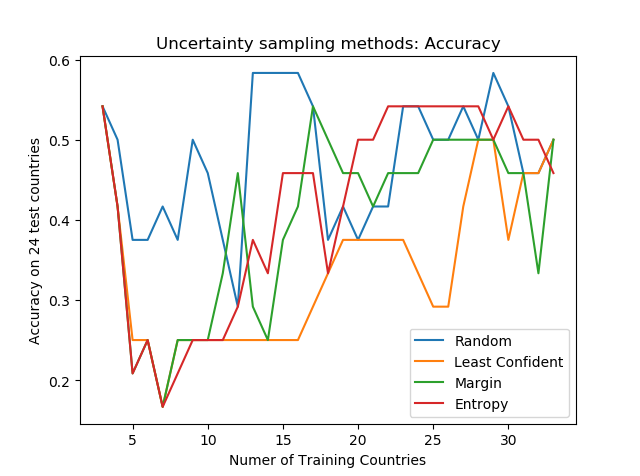
\includegraphics[width=\linewidth]{../src/saved_data/Accuracies}
			\caption{The accuracies of all four uncertainty sampling methods for every iteration.}
			\label{fig:accuracies}
		\end{minipage}%
		\begin{minipage}{.5\textwidth}
			\centering
			\includegraphics[width=\linewidth]{"../src/saved_data/Class balancing"}
			\caption{The proportion of the largest class in the pool at each iteration. Balance is at 0.33}
			\label{fig:class-balancing}
		\end{minipage}
		\end{figure}
		
	
\begin{multicols}{2}

	\section{Discussion} %TODO: Write section
		
	% 	
As seen from figure \ref{fig:accuracies}, the four uncertainty sampling methods all seem intertwined. Furthermore, it looks like the random sampling outperforms the proposed methods -- especially early in the query. Somewhat lower performance is seen in the least confident sampling method. This project has no statistic test showing whether the explaining variables describe the number of COVID-19 fatalities accurately, and it is expected that some are redundant or very correlated. Thus, the classification problem might be  unstable and sensitive to outliers which is problematic for the probabilistic model. A more accurate modeling must account for the dependence and inter-connected generative story between the countries.
	
A counter-intuitive effect is seen for all methods where the accuracy is high initially, before falling rapidly and subsequently regaining accuracy. An important effect, which might account for this, is the class imbalance at each time step in the training, see figure \ref{fig:class-balancing}, as all experiments start out with perfectly balanced data sets. Since the number of training countries increases, the uncertainty sampling methods seem to almost fill up an entire class before sampling other classes -- possibly due to one class containing much of the data variability. This problematic imbalance does not affect random sampling in the same way and might account for its' better early performance.
		
		
\section{Learning outcomes} %TODO: Write section
Throughout the process of conducting the experiment and writing the report, a better understanding of the implementation and inner workings of active learning and uncertainty sampling was achieved. The surprising result of random sampling being close to on par with other methods is taken as a warning of very small data-sets with outliers. Realizing this allows for counteractive measures to be taken in the future to uphold class balance or simply to not use active learning for the first few samplings on a noisy problem . Other minutia like increasing number of Gaussian Process hyperparameter optimizer restarts and using an appropriate kernel also proved important in striving for sensible convergence.
		
\end{multicols}

\newpage
\begin{thebibliography}{9}


	
	\bibitem{density} Wikipedia contributors: "List of countries and dependencies by population density", Date of last revision: 22 March 2020 15:25 UTC. Visited at,  \url{ https://en.wikipedia.org/w/index.php?title=List_of_countries_and_dependencies_by_population_density&oldid=946809073}
	
	\bibitem{corona} Balaaje from Kaggle: "Coronavirus (COVID-19) dataset" with data from \url{https://www.worldometers.info/coronavirus/}. Visited at, \url{https://www.kaggle.com/balaaje/coronavirus-covid19-dataset}
	
	\bibitem{alder} World Population Review: "Countries by Median Age 2018". Visited at, \url{https://worldpopulationreview.com/countries/median-age/}
	
	\bibitem{bnp} International Monetary Fund: "GDP per capita, current prices", ©IMF, 2019. Visited at, \url{https://www.imf.org/external/datamapper/NGDPDPC@WEO/OEMDC/ADVEC/WEOWORLD}
	
	\bibitem{region} J. SnowLabs, Datahub.io: "Country and Continent Codes List" . Can be found at, \url{https://datahub.io/JohnSnowLabs/country-and-continent-codes-list}
	
	\bibitem{healthcare} Numbeo.com: "Health Care Index by Country 2020". Visited at, \url{https://www.numbeo.com/health-care/rankings_by_country.jsp}
	
	\bibitem{turist} World Economic Forum: "Travel and Tourism Competitiveness Index", © 2020 World Economic Forum. Visited at, \url{http://reports.weforum.org/travel-and-tourism-competitiveness-report-2019/rankings/}
	
	
	
	
	
\end{thebibliography}

%\section{Appendix}


\end{document}

















